\chapter{完整搜索}

\key{完整搜索}是一种几乎可用于解决任何算法问题的通用方法。其思想是用暴力方法生成所有可能解，再根据题意选出最优解或统计解的数量。

若有足够时间遍历全部解，完整搜索是很好的技术，因为它通常易于实现且一定能得到正确答案。若完整搜索太慢，则需要贪心、动态规划等其他技术。

\section{生成子集}

\index{subset}

首先考虑生成一个 $n$ 元集合的全部子集。例如，$\{0,1,2\}$ 的子集为
$\emptyset$, $\{0\}$, $\{1\}$, $\{2\}$, $\{0,1\}$,
$\{0,2\}$, $\{1,2\}$ and $\{0,1,2\}$.
生成子集有两种常见方法：递归搜索，或利用整数的二进制表示。

\subsubsection{方法一}

一种优雅的子集遍历方式是递归。下面的函数 \texttt{search} 生成集合 $\{0,1,\ldots,n-1\}$ 的全部子集。函数维护向量 \texttt{subset} 存放当前子集元素，从参数 0 开始调用。

\begin{lstlisting}
void search(int k) {
    if (k == n) {
        // process subset
    } else {
        search(k+1);
        subset.push_back(k);
        search(k+1);
        subset.pop_back();
    }
}
\end{lstlisting}

调用 \texttt{search}$(k)$ 时，函数决定是否把元素 $k$ 加入子集，两种情况下都再以 $k+1$ 递归调用自身。若 $k=n$，说明所有元素均已处理，一个子集生成完毕。

下图展示 $n=3$ 时的函数调用。每次可选择左分支（不加入 $k$）或右分支（加入 $k$）。

\begin{center}
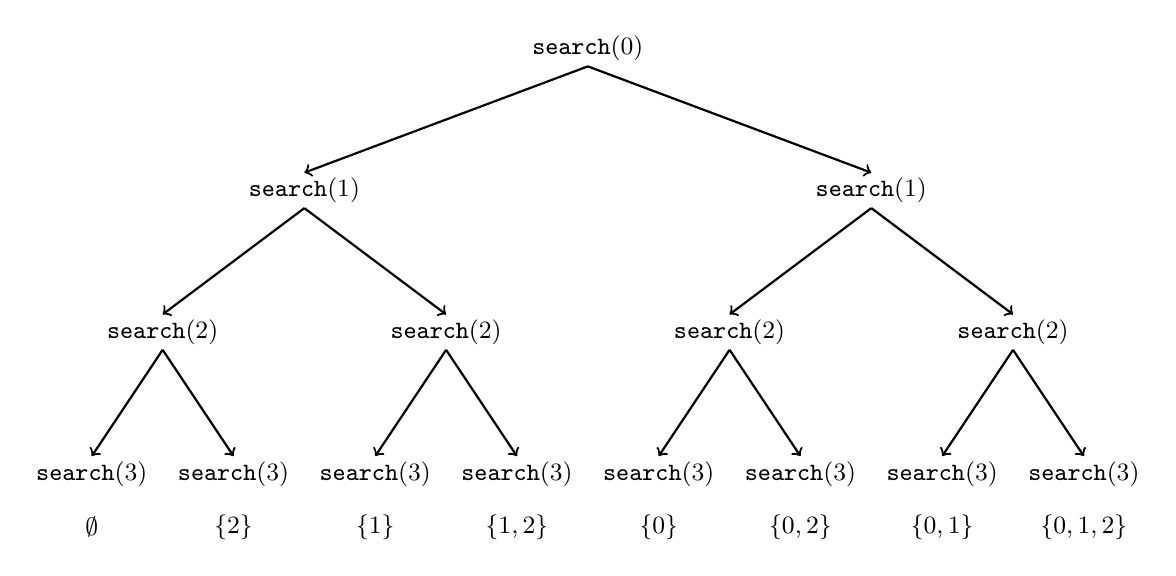
\begin{tikzpicture}[scale=.45]
  \begin{scope}
    \small
    \node at (0,0) {$\texttt{search}(0)$};

    \node at (-8,-4) {$\texttt{search}(1)$};
    \node at (8,-4) {$\texttt{search}(1)$};

    \path[draw,thick,->] (0,0-0.5) -- (-8,-4+0.5);
    \path[draw,thick,->] (0,0-0.5) -- (8,-4+0.5);

    \node at (-12,-8) {$\texttt{search}(2)$};
    \node at (-4,-8) {$\texttt{search}(2)$};
    \node at (4,-8) {$\texttt{search}(2)$};
    \node at (12,-8) {$\texttt{search}(2)$};

    \path[draw,thick,->] (-8,-4-0.5) -- (-12,-8+0.5);
    \path[draw,thick,->] (-8,-4-0.5) -- (-4,-8+0.5);
    \path[draw,thick,->] (8,-4-0.5) -- (4,-8+0.5);
    \path[draw,thick,->] (8,-4-0.5) -- (12,-8+0.5);

    \node at (-14,-12) {$\texttt{search}(3)$};
    \node at (-10,-12) {$\texttt{search}(3)$};
    \node at (-6,-12) {$\texttt{search}(3)$};
    \node at (-2,-12) {$\texttt{search}(3)$};
    \node at (2,-12) {$\texttt{search}(3)$};
    \node at (6,-12) {$\texttt{search}(3)$};
    \node at (10,-12) {$\texttt{search}(3)$};
    \node at (14,-12) {$\texttt{search}(3)$};

    \node at (-14,-13.5) {$\emptyset$};
    \node at (-10,-13.5) {$\{2\}$};
    \node at (-6,-13.5) {$\{1\}$};
    \node at (-2,-13.5) {$\{1,2\}$};
    \node at (2,-13.5) {$\{0\}$};
    \node at (6,-13.5) {$\{0,2\}$};
    \node at (10,-13.5) {$\{0,1\}$};
    \node at (14,-13.5) {$\{0,1,2\}$};


    \path[draw,thick,->] (-12,-8-0.5) -- (-14,-12+0.5);
    \path[draw,thick,->] (-12,-8-0.5) -- (-10,-12+0.5);
    \path[draw,thick,->] (-4,-8-0.5) -- (-6,-12+0.5);
    \path[draw,thick,->] (-4,-8-0.5) -- (-2,-12+0.5);
    \path[draw,thick,->] (4,-8-0.5) -- (2,-12+0.5);
    \path[draw,thick,->] (4,-8-0.5) -- (6,-12+0.5);
    \path[draw,thick,->] (12,-8-0.5) -- (10,-12+0.5);
    \path[draw,thick,->] (12,-8-0.5) -- (14,-12+0.5);
\end{scope}
\end{tikzpicture}
\end{center}

\subsubsection{方法二}

另一种方法基于整数的二进制表示。$n$ 元集合的每个子集都可表示为长度为 $n$ 的二进制序列，对应 $0 \ldots 2^n-1$ 之间的整数；序列中的 1 表示哪些元素属于子集。

通常规定最低位对应元素 0，次低位对应元素 1，依此类推。例如，25 的二进制表示为 11001，对应子集 $\{0,3,4\}$。

下面的代码遍历 $n$ 元集合的所有子集：

\begin{lstlisting}
for (int b = 0; b < (1<<n); b++) {
    // process subset
}
\end{lstlisting}

下面展示如何找出一个二进制序列对应子集中的元素。处理每个子集时，代码构造一个向量保存其中元素。

\begin{lstlisting}
for (int b = 0; b < (1<<n); b++) {
    vector<int> subset;
    for (int i = 0; i < n; i++) {
        if (b&(1<<i)) subset.push_back(i);
    }
}
\end{lstlisting}

\section{生成排列}

\index{permutation}

下面考虑生成 $n$ 元集合的全部排列。例如，$\{0,1,2\}$ 的排列为
$(0,1,2)$, $(0,2,1)$, $(1,0,2)$, $(1,2,0)$,
$(2,0,1)$ and $(2,1,0)$.
同样有两种方法：递归生成，或迭代遍历排列。

\subsubsection{方法一}

与子集一样，排列也可递归生成。下面的 \texttt{search} 遍历集合 $\{0,1,\ldots,n-1\}$ 的排列，并在向量 \texttt{permutation} 中构造当前排列；搜索从无参数调用开始。

\begin{lstlisting}
void search() {
    if (permutation.size() == n) {
        // process permutation
    } else {
        for (int i = 0; i < n; i++) {
            if (chosen[i]) continue;
            chosen[i] = true;
            permutation.push_back(i);
            search();
            chosen[i] = false;
            permutation.pop_back();
        }
    }
}
\end{lstlisting}

每次函数调用向 \texttt{permutation} 加入一个新元素。数组 \texttt{chosen} 记录哪些元素已在排列中。当 \texttt{permutation} 大小等于集合大小时，一个排列生成完毕。

\subsubsection{方法二}

\index{next\_permutation@\texttt{next\_permutation}}

另一种方法从排列 $\{0,1,\ldots,n-1\}$ 开始，反复调用函数构造字典序中的下一个排列。C++ 标准库提供 \texttt{next\_permutation}：

\begin{lstlisting}
vector<int> permutation;
for (int i = 0; i < n; i++) {
    permutation.push_back(i);
}
do {
    // process permutation
} while (next_permutation(permutation.begin(),permutation.end()));
\end{lstlisting}

\section{回溯法}

\index{backtracking}

\key{回溯法}从一个空解开始，逐步扩展这个解。搜索过程递归地遍历构造解的所有不同方式。

\index{queen problem}

例如，考虑计算在 $n \times n$ 的棋盘上放置 $n$ 个皇后且任意两个皇后互不攻击的方案数。当 $n=4$ 时，有两种可能的解：

\begin{center}
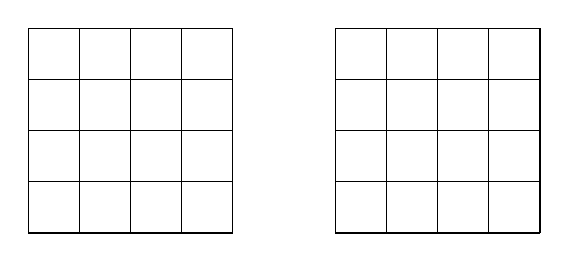
\begin{tikzpicture}[scale=.65]
  \begin{scope}
    \draw (0, 0) grid (4, 4);
    \node at (1.5,3.5) {\symqueen};
    \node at (3.5,2.5) {\symqueen};
    \node at (0.5,1.5) {\symqueen};
    \node at (2.5,0.5) {\symqueen};

    \draw (6, 0) grid (10, 4);
    \node at (6+2.5,3.5) {\symqueen};
    \node at (6+0.5,2.5) {\symqueen};
    \node at (6+3.5,1.5) {\symqueen};
    \node at (6+1.5,0.5) {\symqueen};

  \end{scope}
\end{tikzpicture}
\end{center}

可以使用回溯法逐行在棋盘上放置皇后来解决这个问题。更准确地说，每一行恰好放置一个皇后，并保证它不会攻击此前放置的任何皇后。当 $n$ 个皇后都已放到棋盘上时，就找到了一个解。

例如，当 $n=4$ 时，回溯算法生成的一些部分解如下：

\begin{center}
\begin{tikzpicture}[scale=.55]
  \begin{scope}
    \draw (0, 0) grid (4, 4);

    \draw (-9, -6) grid (-5, -2);
    \draw (-3, -6) grid (1, -2);
    \draw (3, -6) grid (7, -2);
    \draw (9, -6) grid (13, -2);

    \node at (-9+0.5,-3+0.5) {\symqueen};
    \node at (-3+1+0.5,-3+0.5) {\symqueen};
    \node at (3+2+0.5,-3+0.5) {\symqueen};
    \node at (9+3+0.5,-3+0.5) {\symqueen};

    \draw (2,0) -- (-7,-2);
    \draw (2,0) -- (-1,-2);
    \draw (2,0) -- (5,-2);
    \draw (2,0) -- (11,-2);

    \draw (-11, -12) grid (-7, -8);
    \draw (-6, -12) grid (-2, -8);
    \draw (-1, -12) grid (3, -8);
    \draw (4, -12) grid (8, -8);
    \draw[white] (11, -12) grid (15, -8);
    \node at (-11+1+0.5,-9+0.5) {\symqueen};
    \node at (-6+1+0.5,-9+0.5) {\symqueen};
    \node at (-1+1+0.5,-9+0.5) {\symqueen};
    \node at (4+1+0.5,-9+0.5) {\symqueen};
    \node at (-11+0+0.5,-10+0.5) {\symqueen};
    \node at (-6+1+0.5,-10+0.5) {\symqueen};
    \node at (-1+2+0.5,-10+0.5) {\symqueen};
    \node at (4+3+0.5,-10+0.5) {\symqueen};

    \draw (-1,-6) -- (-9,-8);
    \draw (-1,-6) -- (-4,-8);
    \draw (-1,-6) -- (1,-8);
    \draw (-1,-6) -- (6,-8);

    \node at (-9,-13) {非法};
    \node at (-4,-13) {非法};
    \node at (1,-13) {非法};
    \node at (6,-13) {合法};

  \end{scope}
\end{tikzpicture}
\end{center}

在最下层，前三种布局都是非法的，因为其中的皇后会互相攻击。第四种布局则是合法的；再向棋盘放置两个皇后即可将其扩展为完整解，而这两个剩余皇后的放置方式只有一种。

\begin{samepage}
该算法可以实现如下：
\begin{lstlisting}
void search(int y) {
    if (y == n) {
        count++;
        return;
    }
    for (int x = 0; x < n; x++) {
        if (column[x] || diag1[x+y] || diag2[x-y+n-1]) continue;
        column[x] = diag1[x+y] = diag2[x-y+n-1] = 1;
        search(y+1);
        column[x] = diag1[x+y] = diag2[x-y+n-1] = 0;
    }
}
\end{lstlisting}
\end{samepage}
搜索从调用 \texttt{search(0)} 开始。棋盘大小为 $n \times n$，代码将解的数量计算到 \texttt{count} 中。

代码假设棋盘的行和列均从 0 编号到 $n-1$。以参数 $y$ 调用函数 \texttt{search} 时，它会在第 $y$ 行放置一个皇后，然后以参数 $y+1$ 递归调用自身。当 $y=n$ 时，说明已经找到一个解，于是变量 \texttt{count} 加一。

数组 \texttt{column} 记录哪些列中已有皇后，数组 \texttt{diag1} 和 \texttt{diag2} 则记录两组对角线。不能在已经包含皇后的列或对角线上再放置皇后。例如，$4 \times 4$ 棋盘的列和对角线编号如下：

\begin{center}
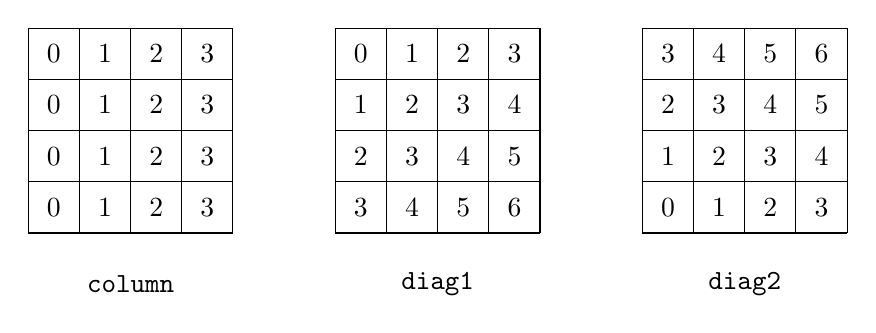
\begin{tikzpicture}[scale=.65]
  \begin{scope}
    \draw (0-6, 0) grid (4-6, 4);
    \node at (-6+0.5,3.5) {$0$};
    \node at (-6+1.5,3.5) {$1$};
    \node at (-6+2.5,3.5) {$2$};
    \node at (-6+3.5,3.5) {$3$};
    \node at (-6+0.5,2.5) {$0$};
    \node at (-6+1.5,2.5) {$1$};
    \node at (-6+2.5,2.5) {$2$};
    \node at (-6+3.5,2.5) {$3$};
    \node at (-6+0.5,1.5) {$0$};
    \node at (-6+1.5,1.5) {$1$};
    \node at (-6+2.5,1.5) {$2$};
    \node at (-6+3.5,1.5) {$3$};
    \node at (-6+0.5,0.5) {$0$};
    \node at (-6+1.5,0.5) {$1$};
    \node at (-6+2.5,0.5) {$2$};
    \node at (-6+3.5,0.5) {$3$};

    \draw (0, 0) grid (4, 4);
    \node at (0.5,3.5) {$0$};
    \node at (1.5,3.5) {$1$};
    \node at (2.5,3.5) {$2$};
    \node at (3.5,3.5) {$3$};
    \node at (0.5,2.5) {$1$};
    \node at (1.5,2.5) {$2$};
    \node at (2.5,2.5) {$3$};
    \node at (3.5,2.5) {$4$};
    \node at (0.5,1.5) {$2$};
    \node at (1.5,1.5) {$3$};
    \node at (2.5,1.5) {$4$};
    \node at (3.5,1.5) {$5$};
    \node at (0.5,0.5) {$3$};
    \node at (1.5,0.5) {$4$};
    \node at (2.5,0.5) {$5$};
    \node at (3.5,0.5) {$6$};

    \draw (6, 0) grid (10, 4);
    \node at (6.5,3.5) {$3$};
    \node at (7.5,3.5) {$4$};
    \node at (8.5,3.5) {$5$};
    \node at (9.5,3.5) {$6$};
    \node at (6.5,2.5) {$2$};
    \node at (7.5,2.5) {$3$};
    \node at (8.5,2.5) {$4$};
    \node at (9.5,2.5) {$5$};
    \node at (6.5,1.5) {$1$};
    \node at (7.5,1.5) {$2$};
    \node at (8.5,1.5) {$3$};
    \node at (9.5,1.5) {$4$};
    \node at (6.5,0.5) {$0$};
    \node at (7.5,0.5) {$1$};
    \node at (8.5,0.5) {$2$};
    \node at (9.5,0.5) {$3$};

    \node at (-4,-1) {\texttt{column}};
    \node at (2,-1) {\texttt{diag1}};
    \node at (8,-1) {\texttt{diag2}};

  \end{scope}
\end{tikzpicture}
\end{center}

令 $q(n)$ 表示在 $n \times n$ 棋盘上放置 $n$ 个皇后的方案数。上述回溯算法告诉我们，例如 $q(8)=92$。随着 $n$ 增大，搜索会迅速变慢，因为解的数量呈指数增长。例如，在现代计算机上使用上述算法计算 $q(16)=14772512$ 已经需要约一分钟\footnote{目前还没有已知方法能够高效计算更大的 $q(n)$。当前纪录是 2016 年计算出的 $q(27)=234907967154122528$ \cite{q27}。}。

\section{搜索剪枝}

通常可以通过对搜索树进行\key{剪枝}来优化回溯算法。其思想是让算法具备一定的“判断能力”，尽早发现某个部分解无法扩展为完整解。这类优化可能极大提高搜索效率。

考虑这样一个问题：计算 $n \times n$ 网格中从左上角到右下角，并且恰好访问每个方格一次的路径数。例如，在 $7 \times 7$ 网格中共有 111712 条这样的路径，其中一条如下：

\begin{center}
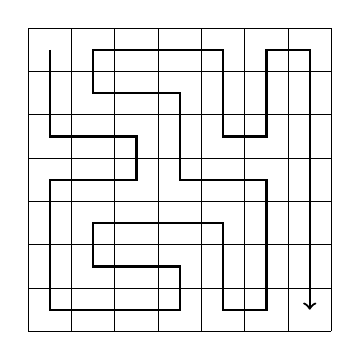
\begin{tikzpicture}[scale=.55]
  \begin{scope}
    \draw (0, 0) grid (7, 7);
    \draw[thick,->] (0.5,6.5) -- (0.5,4.5) -- (2.5,4.5) --
          (2.5,3.5) -- (0.5,3.5) -- (0.5,0.5) --
          (3.5,0.5) -- (3.5,1.5) -- (1.5,1.5) --
          (1.5,2.5) -- (4.5,2.5) -- (4.5,0.5) --
          (5.5,0.5) -- (5.5,3.5) -- (3.5,3.5) --
          (3.5,5.5) -- (1.5,5.5) -- (1.5,6.5) --
          (4.5,6.5) -- (4.5,4.5) -- (5.5,4.5) --
          (5.5,6.5) -- (6.5,6.5) -- (6.5,0.5);
  \end{scope}
\end{tikzpicture}
\end{center}

我们重点研究 $7 \times 7$ 的情形，因为它的难度恰好适合这里的需要。先从一个直接的回溯算法开始，再根据对剪枝方式的观察逐步优化。每次优化后，我们都会测量算法运行时间与递归调用次数，从而清楚看到各项优化对搜索效率的影响。

\subsubsection{基本算法}

算法的第一个版本不包含任何优化。我们只是使用回溯法生成从左上角到右下角的所有可能路径，并统计其数量。

\begin{itemize}
\item
运行时间：483 秒
\item
递归调用次数：760 亿
\end{itemize}

\subsubsection{优化一}

在任意解中，第一步都只能向下或向右走。第一步之后，路径总能按网格的对角线找到一条对称路径。例如，下列两条路径互为对称：

\begin{center}
\begin{tabular}{ccc}
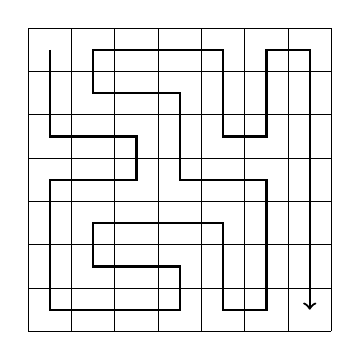
\begin{tikzpicture}[scale=.55]
  \begin{scope}
    \draw (0, 0) grid (7, 7);
    \draw[thick,->] (0.5,6.5) -- (0.5,4.5) -- (2.5,4.5) --
          (2.5,3.5) -- (0.5,3.5) -- (0.5,0.5) --
          (3.5,0.5) -- (3.5,1.5) -- (1.5,1.5) --
          (1.5,2.5) -- (4.5,2.5) -- (4.5,0.5) --
          (5.5,0.5) -- (5.5,3.5) -- (3.5,3.5) --
          (3.5,5.5) -- (1.5,5.5) -- (1.5,6.5) --
          (4.5,6.5) -- (4.5,4.5) -- (5.5,4.5) --
          (5.5,6.5) -- (6.5,6.5) -- (6.5,0.5);
  \end{scope}
\end{tikzpicture}
& \hspace{20pt}
& 
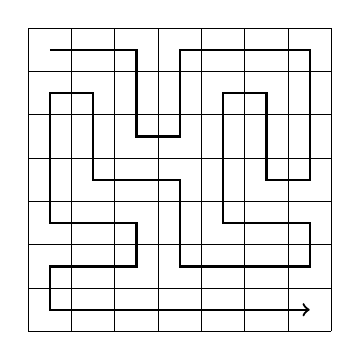
\begin{tikzpicture}[scale=.55]
  \begin{scope}[yscale=1,xscale=-1,rotate=-90]
    \draw (0, 0) grid (7, 7);
    \draw[thick,->] (0.5,6.5) -- (0.5,4.5) -- (2.5,4.5) --
          (2.5,3.5) -- (0.5,3.5) -- (0.5,0.5) --
          (3.5,0.5) -- (3.5,1.5) -- (1.5,1.5) --
          (1.5,2.5) -- (4.5,2.5) -- (4.5,0.5) --
          (5.5,0.5) -- (5.5,3.5) -- (3.5,3.5) --
          (3.5,5.5) -- (1.5,5.5) -- (1.5,6.5) --
          (4.5,6.5) -- (4.5,4.5) -- (5.5,4.5) --
          (5.5,6.5) -- (6.5,6.5) -- (6.5,0.5);
  \end{scope}
\end{tikzpicture}
\end{tabular}
\end{center}

因此，可以规定第一步总是向下（或向右），最后再将解的数量乘以二。

\begin{itemize}
\item
运行时间：244 秒
\item
递归调用次数：380 亿
\end{itemize}

\subsubsection{优化二}

如果路径在访问网格的所有其他方格之前就到达右下角，那么显然不可能再完成这个解。下面的路径就是一例：

\begin{center}
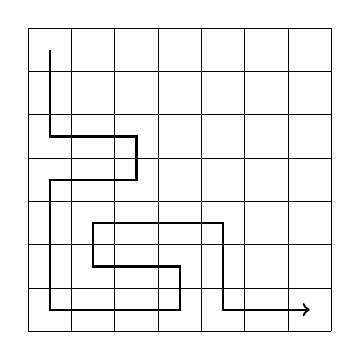
\begin{tikzpicture}[scale=.55]
  \begin{scope}
    \draw (0, 0) grid (7, 7);
    \draw[thick,->] (0.5,6.5) -- (0.5,4.5) -- (2.5,4.5) --
          (2.5,3.5) -- (0.5,3.5) -- (0.5,0.5) --
          (3.5,0.5) -- (3.5,1.5) -- (1.5,1.5) --
          (1.5,2.5) -- (4.5,2.5) -- (4.5,0.5) --
          (6.5,0.5);
  \end{scope}
\end{tikzpicture}
\end{center}
利用这一观察，如果过早到达右下角，就可以立即终止搜索。
\begin{itemize}
\item
运行时间：119 秒
\item
递归调用次数：200 亿
\end{itemize}

\subsubsection{优化三}

如果路径抵达边界，并且既可以向左转也可以向右转，那么网格会被分成两个都含有未访问方格的部分。例如，在下列情形中，路径可以向左转或向右转：

\begin{center}
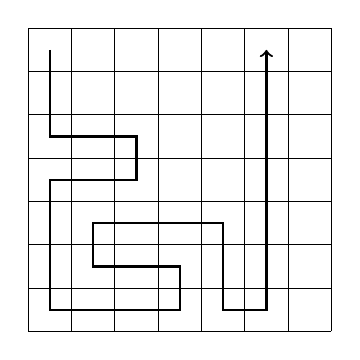
\begin{tikzpicture}[scale=.55]
  \begin{scope}
    \draw (0, 0) grid (7, 7);
    \draw[thick,->] (0.5,6.5) -- (0.5,4.5) -- (2.5,4.5) --
          (2.5,3.5) -- (0.5,3.5) -- (0.5,0.5) --
          (3.5,0.5) -- (3.5,1.5) -- (1.5,1.5) --
          (1.5,2.5) -- (4.5,2.5) -- (4.5,0.5) --
          (5.5,0.5) -- (5.5,6.5);
  \end{scope}
\end{tikzpicture}
\end{center}
在这种情况下，已经无法访问所有方格，因此可以终止搜索。这项优化非常有效：

\begin{itemize}
\item
运行时间：1.8 秒
\item
递归调用次数：2.21 亿
\end{itemize}

\subsubsection{优化四}

优化三的思想还可以推广：如果路径无法继续向前，却既可以向左转也可以向右转，那么网格同样会被分成两个都含有未访问方格的部分。例如，考虑下面的路径：

\begin{center}
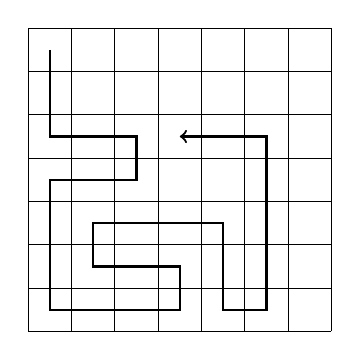
\begin{tikzpicture}[scale=.55]
  \begin{scope}
    \draw (0, 0) grid (7, 7);
    \draw[thick,->] (0.5,6.5) -- (0.5,4.5) -- (2.5,4.5) --
          (2.5,3.5) -- (0.5,3.5) -- (0.5,0.5) --
          (3.5,0.5) -- (3.5,1.5) -- (1.5,1.5) --
          (1.5,2.5) -- (4.5,2.5) -- (4.5,0.5) --
          (5.5,0.5) -- (5.5,4.5) -- (3.5,4.5);
  \end{scope}
\end{tikzpicture}
\end{center}
显然，此时已经无法访问所有方格，因此可以终止搜索。经过这项优化后，搜索已经非常高效：

\begin{itemize}
\item
运行时间：0.6 秒
\item
递归调用次数：6900 万
\end{itemize}

~\\
现在正适合暂停优化，看看已经取得的成果。原始算法的运行时间是 483 秒，而经过这些优化后，运行时间仅为 0.6 秒。也就是说，优化后的算法速度提升了将近 1000 倍。

这在回溯算法中很常见：搜索树通常很大，即使简单的观察也能有效剪枝。尤其有用的是那些能在算法最初几步、也就是搜索树顶部生效的优化。

\section{折半搜索}

\index{meet in the middle}

\key{折半搜索}是一种将搜索空间划分为两个大小大致相等的部分，分别搜索两部分，最后合并搜索结果的技术。

如果能够高效合并两次搜索的结果，就可以使用这种技术。在这种情况下，两次较小搜索所需的时间可能少于一次大搜索。通常，折半搜索可以把 $2^n$ 这一因子降为 $2^{n/2}$。

例如，给定一个包含 $n$ 个数的列表以及一个数 $x$，我们希望判断能否从列表中选出若干数，使它们的和为 $x$。对于列表 $[2,4,5,9]$ 和 $x=15$，可以选择 $[2,4,9]$，得到 $2+4+9=15$。但对于同一个列表，如果 $x=10$，就无法凑出这个和。

解决该问题的一种简单算法是遍历所有元素子集，检查是否有某个子集的元素和等于 $x$。由于共有 $2^n$ 个子集，该算法的运行时间为 $O(2^n)$。使用折半搜索则可以得到更高效的 $O(2^{n/2})$ 时间算法\footnote{这一思想由 E. Horowitz 和 S. Sahni 于 1974 年提出 \cite{hor74}。}。注意，$O(2^n)$ 与 $O(2^{n/2})$ 是不同的复杂度，因为 $2^{n/2}=\sqrt{2^n}$。

其思路是把原列表分为 $A$ 和 $B$ 两个列表，使二者各包含约一半的数。第一次搜索生成 $A$ 的所有子集，并将各子集的元素和存入列表 $S_A$；相应地，第二次搜索由 $B$ 构造列表 $S_B$。之后，只需检查能否分别从 $S_A$ 和 $S_B$ 中各选一个元素，使二者之和为 $x$。这成立当且仅当能用原列表中的数凑出和 $x$。

例如，设列表为 $[2,4,5,9]$，且 $x=15$。首先将其分为 $A=[2,4]$ 和 $B=[5,9]$，再构造 $S_A=[0,2,4,6]$ 与 $S_B=[0,5,9,14]$。这里可以凑出 $x=15$，因为 $S_A$ 中有和 $6$，$S_B$ 中有和 $9$，且 $6+9=15$。这对应于解 $[2,4,9]$。

可以将该算法实现为 $O(2^{n/2})$ 时间复杂度。首先生成\emph{有序的}列表 $S_A$ 和 $S_B$，利用类似归并的技术可以在 $O(2^{n/2})$ 时间内完成。此后，由于两个列表已有序，可以在 $O(2^{n/2})$ 时间内检查能否从 $S_A$ 和 $S_B$ 中选出两个数凑成 $x$。
